% Big-GEM / Zenith final technical report.
% Created from the current implementation and measured evidence; the previous
% project report is intentionally not used as a technical source.
\documentclass[11pt,a4paper]{article}

\usepackage[left=22mm,right=22mm,top=22mm,bottom=23mm,headheight=24pt,headsep=7mm,footskip=12mm]{geometry}
\usepackage[T1]{fontenc}
\usepackage[utf8]{inputenc}
\usepackage{lmodern}
\usepackage{microtype}
\usepackage{xcolor}
\definecolor{paper}{HTML}{FBF8F1}
\definecolor{scarlet}{HTML}{B21E2B}
\definecolor{scarletDark}{HTML}{7D1420}
\definecolor{gold}{HTML}{C9A44A}
\definecolor{goldLight}{HTML}{EFE2B9}
\definecolor{softGray}{HTML}{EDE9DF}
\pagecolor{paper}
\color{black}

\usepackage{graphicx}
\usepackage{booktabs}
\usepackage{tabularx}
\usepackage{longtable}
\usepackage{array}
\usepackage{multirow}
\usepackage{enumitem}
\usepackage{makecell}
\usepackage{ragged2e}
\usepackage{amsmath}
\usepackage{amssymb}
\usepackage{tikz}
\usetikzlibrary{arrows.meta,positioning,shapes.geometric,fit,calc,backgrounds}
\usepackage[most]{tcolorbox}
\usepackage{fancyhdr}
\usepackage{titlesec}
\usepackage{caption}
\usepackage{float}
\usepackage{url}
\usepackage[hidelinks]{hyperref}
\usepackage[nameinlink,noabbrev]{cleveref}

\hypersetup{
  colorlinks=false,
  hidelinks,
  pdftitle={Big-GEM: Heterogeneous GPU-Accelerated RTL Simulation},
  pdfauthor={Pratham Sharma and the Big-GEM Team}
}

\setlength{\parindent}{0pt}
\setlength{\parskip}{6pt}
\renewcommand{\arraystretch}{1.22}
\setlist[itemize]{leftmargin=*,itemsep=2pt,topsep=2pt}
\setlist[enumerate]{leftmargin=*,itemsep=3pt,topsep=2pt}

\pagestyle{fancy}
\fancyhf{}
\lhead{\textbf{BIG-GEM THEORY}}
\rhead{Technical Project Report}
\cfoot{\thepage}
\renewcommand{\headrulewidth}{0.5pt}
\renewcommand{\headrule}{\hbox to\headwidth{\color{gold}\leaders\hrule height \headrulewidth\hfill}}

\titleformat{\section}{\Large\bfseries\color{black}}{\thesection.}{0.6em}{}[\vspace{2pt}\color{gold}\titlerule]
\titleformat{\subsection}{\large\bfseries\color{black}}{\thesubsection}{0.6em}{}
\titleformat{\subsubsection}{\normalsize\bfseries\color{black}}{\thesubsubsection}{0.6em}{}
\titlespacing*{\section}{0pt}{16pt}{8pt}
\titlespacing*{\subsection}{0pt}{12pt}{5pt}
\titlespacing*{\subsubsection}{0pt}{9pt}{4pt}

\newtcolorbox{infobox}{enhanced,breakable,colback=white,colframe=gold,boxrule=0.8pt,arc=2mm,left=5mm,right=5mm,top=3mm,bottom=3mm,borderline west={2.5pt}{0pt}{scarlet},coltext=black}
\newtcolorbox{warningbox}{enhanced,breakable,colback=goldLight!35,colframe=scarlet,boxrule=0.7pt,arc=2mm,left=5mm,right=5mm,top=3mm,bottom=3mm,coltext=black}
\newcolumntype{Y}{>{\RaggedRight\arraybackslash}X}
\newcolumntype{P}[1]{>{\RaggedRight\arraybackslash}p{#1}}
\newcolumntype{C}[1]{>{\Centering\arraybackslash}p{#1}}
\newcommand{\code}[1]{\texttt{\detokenize{#1}}}
\newcommand{\verified}{\textbf{Verified}}
\newcommand{\partialstatus}{\textbf{Partial}}
\newcommand{\unverified}{\textbf{Unverified}}

\begin{document}

% ---------------------------------------------------------------------
% Full-page cover, retaining the supplied template's visual convention.
% ---------------------------------------------------------------------
\thispagestyle{empty}

\begin{tikzpicture}[remember picture,overlay]
  \fill[scarletDark] (current page.south west) rectangle (current page.north east);
  \fill[gold] ([xshift=18mm]current page.south west) rectangle ([xshift=24mm]current page.north west);
  \draw[gold,line width=1.2pt] ([xshift=34mm,yshift=-36mm]current page.north west) -- ([xshift=-24mm,yshift=-36mm]current page.north east);
  \node[anchor=north west,text width=150mm,align=left,text=white] at ([xshift=34mm,yshift=-55mm]current page.north west) {
    {\fontsize{34}{39}\selectfont\bfseries BIG-GEM}\par\vspace{3mm}
    {\fontsize{20}{25}\selectfont The Big-GEM Theory}\par\vspace{9mm}
    {\Large Heterogeneous GPU-Accelerated RTL Simulation}\par\vspace{4mm}
    {\large Native DSP48E2, CARRY4, and SRLC32E execution in NVIDIA GEM}
  };
  \node[draw=gold,rounded corners=2mm,line width=1pt,fill=white,text=scarletDark,
        text width=122mm,minimum height=42mm,align=center] at ([yshift=-5mm]current page.center) {
    {\Large\bfseries Technical Project Report}\\[4mm]
    {\normalsize Takneek PS -- Zenith}\\[1.5mm]
    {\normalsize Deliverable E}
  };
  \node[anchor=south west,text=white,align=left,text width=145mm] at ([xshift=34mm,yshift=32mm]current page.south west) {
    \textbf{Repository:} \url{https://github.com/Pratham-015/GEM}\\[1.5mm]
    \textbf{Measured revision:} \code{23fc43fac59f2ba6e349132e632cbcb062a1f39b}\\[1.5mm]
    \textbf{Report date:} 2 September 2026
  };
\end{tikzpicture}
\clearpage

\begin{infobox}
\textbf{Project:} Big-GEM / The Big-GEM Theory\\
\textbf{Base system:} NVIDIA GEM GPU-accelerated RTL simulator\\
\textbf{Extension:} Heterogeneous native execution of DSP48E2, CARRY4, and SRLC32E\\
\textbf{Primary measured platform:} NVIDIA GeForce RTX 4050 Laptop GPU (SM 8.9)\\
\textbf{Author recorded in the measured revision:} Pratham Sharma
\end{infobox}

\tableofcontents
\newpage

% =========================================================
\section{Project Overview}
% =========================================================

\subsection{Abstract}

Big-GEM extends NVIDIA GEM from a homogeneous one-bit And-Inverter Graph (AIG)
simulator into a heterogeneous simulator that preserves and executes three FPGA
primitives: DSP48E2, CARRY4, and SRLC32E.  Yosys 0.68 and its Slang frontend
elaborate SystemVerilog while black-box interception and a DSP-specific techmap
retain macro identity.  The host constructs explicit named-port macro records,
classifies same-cycle and clock-boundary dependencies, fuses legal CARRY4 chains,
and creates warp-padded 64-bit structure-of-arrays buffers.  A custom cooperative
CUDA kernel interleaves original Boomerang Boolean propagation with typed macro
gather, shared-memory staging, native 64-bit evaluation, output publication, and a
single synchronized state-commit boundary.

Correctness was tested through the production RTL-to-CUDA path and against
independent Python, literal SystemVerilog, and installed Xilinx UNISIM models.
CARRY4 covered its complete 1,024-input truth table plus randomized cases; GPU
differential totals were 3,024 CARRY4 slices, 2,009 fused 60-bit chains, 2,336
DSP cycles, and 2,100 SRLC32E cycles.  Four randomized production DAG topologies
and the exact DSP$\rightarrow$CARRY4$\rightarrow$SRLC32E$\rightarrow$DSP chain
matched independent RTL with zero reported mismatches.

Production throughput was measured with 12 warm-ups and seven retained launches.
The only identical-workload comparison supported by both official upstream and
the modified simulator is Boolean-only: 59,232 versus 59,322 simulated cycles/s,
or 1.0015$\times$ (+0.153\%).  A separate 9-partition heterogeneous stress design
scaled from 5,273 cycles/s at one block to 16,677 cycles/s at 12 blocks
(3.163$\times$).  No valid heterogeneous upstream speedup is claimed: the
historical shredded-netlist comparison failed its RTL correctness gate.

\subsection{Problem and Contribution}

The problem statement identifies a structural inefficiency in conventional GEM:
Yosys decomposition converts wide arithmetic and stateful primitives into large
one-bit networks.  Big-GEM changes the representation and execution path rather
than adding an isolated macro microbenchmark.  Its concrete contributions are:

\begin{enumerate}
  \item a Yosys 0.68 macro-preserving and DSP-normalizing frontend;
  \item a heterogeneous host graph with stable port identities, dependency timing,
        and explicit combinational levels;
  \item separate bit-packed Boolean storage and 64-bit aligned, warp-padded macro
        state/I/O storage;
  \item a custom CUDA schedule that places macro operations between Boolean
        settling barriers and commits DSP/SRL state at one global edge; and
  \item reproducible differential, throughput, block-scaling, and Nsight Compute
        evidence.
\end{enumerate}

\begin{warningbox}
\textbf{Evidence boundary.}  Results in this report were regenerated from commit
\code{23fc43f} while the working tree contained the scheduler/benchmark changes
listed by Git as uncommitted.  Every table therefore records the revision and
dirty-tree status.  The repository should be committed and the benchmark command
rerun before final archival publication.
\end{warningbox}

% =========================================================
\section{Requirements and Constraints}
% =========================================================

\begin{table}[H]
\centering
\caption{Problem-statement requirements and demonstrated status.}
\begin{tabularx}{\textwidth}{P{44mm} C{25mm} Y}
\toprule
Requirement & Status & Evidence in the current repository \\
\midrule
Preserve DSP48E2, CARRY4, SRLC32E through Yosys & \verified & Production JSON checks in \path{verif/full_integration_test.py}; Yosys 0.68 observed. \\
Mixed 1-bit and 48-bit heterogeneous scheduling & \verified & Typed dependency graph and production exact-chain/random-DAG differentials. \\
64-bit aligned contiguous macro buffers & \verified & \path{src/macro_layout.rs}; four layout tests, including warp-scale non-overlap. \\
Native GPU ALU macro evaluation & \verified & \path{csrc/gem_macros.cuh} executed on GPU and differentially checked. \\
Correct macro-to-macro sequencing & \verified & Explicit levels; fused CARRY4 chains; exact-chain and randomized production tests. \\
Shared memory and warp synchronization & \verified & 12,288-byte macro tile, \code{__ballot_sync}, block barriers, and cooperative grid barriers. \\
Yosys 0.68 and IEEE 1800-2012 syntax & \verified & Installed Yosys 0.68; Slang parses the SystemVerilog-2012 feature test. \\
Single global clock and zero initialization & \verified & Multiple macro clocks are rejected; state buffers are zero-created and checked. \\
Throughput versus unmodified GEM & \partialstatus & Identical Boolean workload measured; no valid equivalent heterogeneous upstream comparison. \\
Comparison with other pools & \unverified & No attributable external-pool measurements were available. \\
Nsight bandwidth/divergence report & \verified & Four current production-kernel profiles are stored as raw CSV and parsed JSON. \\
\bottomrule
\end{tabularx}
\end{table}

The required DSP configuration is enforced structurally: AREG, BREG, CREG,
DREG, ADREG, and MREG are zero and PREG is one.  Unsupported parameterizations
cause the DSP techmap to fail instead of being silently simulated with different
latency.  The simulator assumes one global clock domain and initializes all
internal macro state to zero; INIT-string parsing remains intentionally out of
scope, exactly as permitted by the problem statement.

% =========================================================
\section{System Architecture}
% =========================================================

\subsection{End-to-End Data Path}

\begin{figure}[H]
\centering
\resizebox{0.98\textwidth}{!}{%
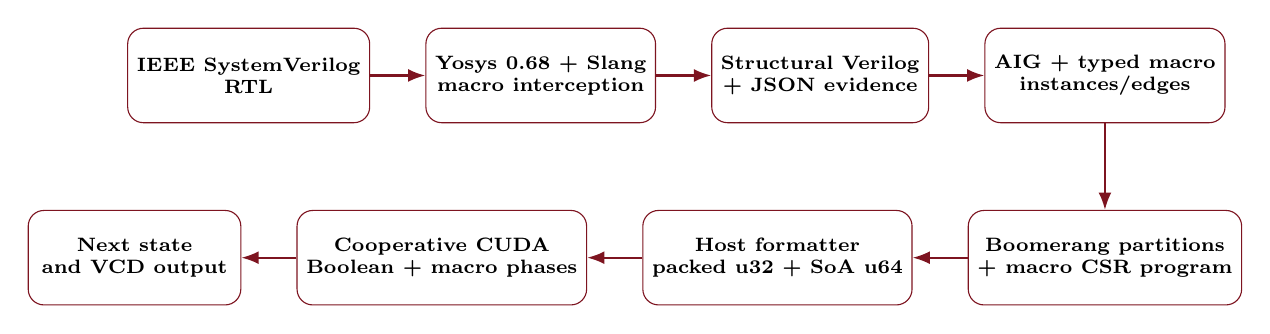
\begin{tikzpicture}[
  node distance=6mm and 7mm,
  box/.style={draw=scarletDark,rounded corners=2mm,fill=white,minimum width=27mm,minimum height=12mm,align=center,font=\scriptsize\bfseries},
  arr/.style={-{Latex[length=2.2mm]},thick,draw=scarletDark}
]
\node[box] (rtl) {IEEE SystemVerilog\\RTL};
\node[box,right=of rtl] (yosys) {Yosys 0.68 + Slang\\macro interception};
\node[box,right=of yosys] (net) {Structural Verilog\\+ JSON evidence};
\node[box,right=of net] (aig) {AIG + typed macro\\instances/edges};
\node[box,below=11mm of aig] (flat) {Boomerang partitions\\+ macro CSR program};
\node[box,left=of flat] (mem) {Host formatter\\packed u32 + SoA u64};
\node[box,left=of mem] (gpu) {Cooperative CUDA\\Boolean + macro phases};
\node[box,left=of gpu] (out) {Next state\\and VCD output};
\draw[arr] (rtl)--(yosys); \draw[arr] (yosys)--(net); \draw[arr] (net)--(aig);
\draw[arr] (aig)--(flat); \draw[arr] (flat)--(mem); \draw[arr] (mem)--(gpu); \draw[arr] (gpu)--(out);
\end{tikzpicture}}
\caption{Actual Big-GEM production path.  No standalone macro microkernel is substituted for the measured simulator.}
\label{fig:pipeline}
\end{figure}

\subsection{Frontend and Macro Preservation}

\path{scripts/synthesize_macros.py} checks the installed version string, invokes
\code{read_slang} with an IEEE 1800-2017 mode that accepts the required 2012
syntax, elaborates the requested top, and runs synthesis/ABC around black-box
macro declarations.  \path{aigpdk/dsp48e2_ps_map.v} transforms a supported raw
DSP48E2 into \code{GEM_DSP48E2} with two state bits and one pre-adder-control
bit.  CARRY4 and SRLC32E remain named black boxes.  JSON is not the runtime
parser input; it is retained as machine-checkable preservation evidence.  The
runtime host parser consumes the emitted structural Verilog and constructs
\code{NetlistDB}, AIG, and macro records.

The DSP control mapping is:
\[
  \operatorname{state}(\mathrm{OPMODE})=
  \begin{cases}
     0,&\mathrm{OPMODE}=\mathtt{0x030},\\
     1,&\mathrm{OPMODE}=\mathtt{0x005},\\
     2,&\mathrm{OPMODE}=\mathtt{0x025},
  \end{cases}
  \qquad
  \operatorname{use\_pre}=\mathrm{INMODE}[2].
\]
Plain-add ALUMODE and supported INMODE encodings are recognized by the map.
Static pipeline parameters outside the required subset are rejected.

% =========================================================
\section{Heterogeneous Graph and Scheduling Equations}
% =========================================================

\subsection{Typed Graph}

Let the execution graph be
\[
  G=(V,E),\qquad
  V=V_B\cup V_C\cup V_S\cup V_D,
\]
where $V_B$ contains one-bit AIG operations, $V_C$ fused CARRY4-chain nodes,
$V_S$ SRLC32E nodes, and $V_D$ DSP48E2 nodes.  The sets are disjoint and each
macro instance retains named input/output ports and bit indices.  Define
\[
  T(v)\in\{\mathrm{AIG},\mathrm{CARRY},\mathrm{SRL},\mathrm{DSP}\}.
\]
An edge records producer cell/port/bit and consumer cell/port/bit.  The frontend
traces through intervening AIG logic, so a macro dependency is recovered even
when ordinary Boolean nodes lie between producer and consumer.

Each macro input has role $r_i\in\{\mathrm{comb},\mathrm{next}\}$ and each
macro output has role $r_o\in\{\mathrm{comb},\mathrm{reg}\}$.  The implemented
timing classifier is exactly
\[
 \tau(e)=
 \begin{cases}
  \mathrm{same}, & r_i(e)=\mathrm{comb}\ \land\ r_o(e)=\mathrm{comb},\\
  \mathrm{edge}, & \text{otherwise}.
 \end{cases}
\]
CARRY O/CO and SRL Q/Q31 are combinational outputs; DSP P is registered.
CARRY inputs and SRL address are combinational; DSP operands/control and SRL
D/CE are next-state inputs.

\subsection{Combinational Levelization}

Only nodes with combinational outputs participate in the same-cycle macro DAG
$G_c=(V_c,E_c)$, where $E_c=\{e\in E:\tau(e)=\mathrm{same}\}$.  The host uses
Kahn levelization.  Its equivalent recurrence is
\[
 \ell(v)=
 \begin{cases}
  0, & \operatorname{pred}_{E_c}(v)=\varnothing,\\
  1+\max\limits_{u\in\operatorname{pred}_{E_c}(v)}\ell(u),&\text{otherwise}.
 \end{cases}
\]
The cohort at level $k$ is $M_k=\{v\in V_c:\ell(v)=k\}$.  A nonempty residual
indegree after Kahn traversal is rejected as a combinational macro cycle.
DSP nodes do not enter $G_c$ because PREG=1 makes P a cycle-boundary source.

Legal adjacent CARRY4 instances are fused before levelization when
CO[3] drives the next CIN, CYINIT is inactive, and total width is at most 60
bits.  For a fused chain, the internal macro-to-macro edges disappear and one
native operation publishes all O/CO bits.  Non-fused same-cycle macro edges are
ordered by $\ell$ and communicated through explicitly allocated output-bit
slots in the packed Boolean-state row.  Thus ordering is explicit, although the
current implementation does not forward a producer's 64-bit register value
directly to a consumer register.

\subsection{Partition and Block Assignment}

For endpoint cone $i$, let $w_i$ be the host-computed fractional AIG work rounded
to an integer.  When the optional external hypergraph partitioner is absent, the
current fallback applies deterministic longest-processing-time assignment:
\[
  i_1,\ldots,i_n=\operatorname{argsort}_{i}(-w_i,i),\qquad
  p(i_j)=\arg\min_{q\in[0,k)}\left(W_q,q\right),
\]
\[
  W_{p(i_j)}\leftarrow W_{p(i_j)}+\max(w_{i_j},1).
\]
Mapping validity remains controlled by \code{Partition::build\_one}; failing
groups are repartitioned until each is legal.  Effective partitions are assigned
to CUDA blocks with a second greedy load rule.  If $d(p)$ is the number of
Boomerang stages in partition $p$, its placement cost is $c(p)=d(p)+3$ and
\[
 b(p)=\arg\min_b L_b,\qquad L_{b(p)}\leftarrow L_{b(p)}+c(p).
\]

\subsection{Per-Cycle Heterogeneous Schedule}

Let $\mathcal{B}(x_t,y)$ denote one complete pass over all major Boolean
Boomerang stages using cycle inputs $x_t$ and mutable output row $y$.  Let
$\mathcal{G}_k$, $\mathcal{E}_k$, and $\mathcal{W}_k$ be macro gather,
evaluate, and publish operations for level $k$.  For state $q_t=(P_t,R_t)$:

\begin{enumerate}
  \item publish old DSP registered outputs $P_t$;
  \item for phase $h=0,1$, and every $k=0,\ldots,K-1$, execute
  \[
    y\leftarrow\mathcal{B}(x_t,y),\quad
    z_k\leftarrow\mathcal{G}_k(y),\quad
    m_k\leftarrow\mathcal{E}_k(z_k,q),\quad
    y\leftarrow\mathcal{W}_k(m_k,y),
  \]
  followed by one final $y\leftarrow\mathcal{B}(x_t,y)$;
  \item between phases ($h=0$ only), gather all DSP and SRL next-state inputs
        from the same settled snapshot and commit the single global edge:
  \[
      q_{t+1}=F(q_t,x_t,y^-);
  \]
  \item phase $h=1$ propagates newly registered P and SRL Q/Q31 values to
        same-cycle observable outputs and downstream next-state inputs.
\end{enumerate}

Every gather/evaluate/publish boundary is separated by a cooperative grid
barrier.  This is a deterministic two-phase level walk, not an unconstrained
Jacobi loop.  Its cost limitation is also explicit: the Boolean network is
re-executed $2(K+1)$ times per simulated cycle for heterogeneous designs.

% =========================================================
\section{GPU Memory Hierarchy and Data Movement}
% =========================================================

\subsection{Layout Equations}

Boolean state remains bit-packed in 32-bit words.  Macro state and I/O occupy
separate CUDA allocations of 64-bit words.  For kind $t$ with $n_t$ instances,
the padded stride is
\[
  s_t=32\left\lceil\frac{n_t}{32}\right\rceil.
\]
The structure-of-arrays address of field $f$ for instance $i$ is
\[
  \operatorname{addr}(t,f,i)=B_t+8\left(f\,s_t+i\right)\quad\text{bytes}.
\]
The allocator uses eight I/O fields for CARRY and DSP and four for SRL.  DSP P
and the SRL's 32-bit state each consume one warp-padded 64-bit state slot;
CARRY is stateless.  CUDA allocations and every field address are therefore
8-byte aligned, and adjacent lanes access adjacent 64-bit words for one field.

\subsection{FPGA Primitive to GPU Hierarchy}

\begin{figure}[H]
\centering
\resizebox{0.97\textwidth}{!}{%
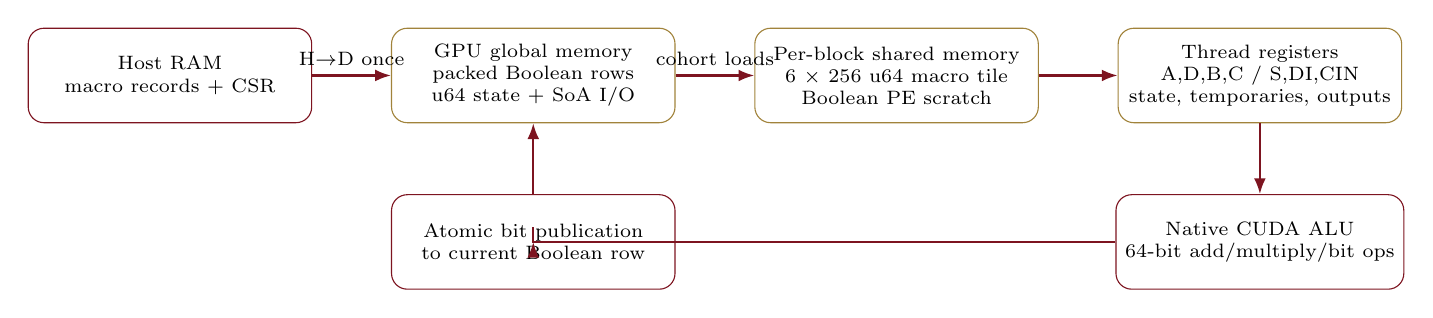
\begin{tikzpicture}[
  box/.style={draw=scarletDark,rounded corners=2mm,fill=white,minimum width=36mm,minimum height=12mm,align=center,font=\scriptsize},
  mem/.style={box,draw=gold!80!black},
  arr/.style={-{Latex[length=2mm]},thick,draw=scarletDark},
  node distance=8mm and 10mm
]
\node[box] (host) {Host RAM\\macro records + CSR};
\node[mem,right=of host] (global) {GPU global memory\\packed Boolean rows\\u64 state + SoA I/O};
\node[mem,right=of global] (shared) {Per-block shared memory\\6 $\times$ 256 u64 macro tile\\Boolean PE scratch};
\node[mem,right=of shared] (regs) {Thread registers\\A,D,B,C / S,DI,CIN\\state, temporaries, outputs};
\node[box,below=9mm of regs] (alu) {Native CUDA ALU\\64-bit add/multiply/bit ops};
\node[box,below=9mm of global] (publish) {Atomic bit publication\\to current Boolean row};
\draw[arr] (host)--node[above,font=\scriptsize]{H$\rightarrow$D once}(global);
\draw[arr] (global)--node[above,font=\scriptsize]{cohort loads}(shared);
\draw[arr] (shared)--(regs); \draw[arr] (regs)--(alu);
\draw[arr] (alu)-|(publish); \draw[arr] (publish)--(global);
\end{tikzpicture}}
\caption{Actual macro data movement.  Global memory is the grid-wide exchange boundary; shared memory is a block-local staging tile; arithmetic temporaries remain in registers.}
\label{fig:memory}
\end{figure}

\begin{table}[H]
\centering
\caption{Primitive-specific mapping onto the measured CUDA hierarchy.}
\begin{tabularx}{\textwidth}{P{24mm} C{20mm} C{17mm} Y Y Y}
\toprule
Primitive & Datapath & State & Global memory & Shared tile & Registers / execution \\
\midrule
DSP48E2 & 27+27, 18, 45, 48 bit & 48-bit P & Five SoA input fields, P state, output bit slots & Five inputs + one state word/thread & Signed 64-bit pre-add, multiply, and masked ALU select \\
CARRY chain & 4--60 bit & None & Three input fields and O/CO output slots & S, DI, CIN words/thread & One 64-bit add plus Boolean transforms \\
SRLC32E & 5-bit address, 1-bit I/O & 32-bit SRL & One packed control field, state word, Q/Q31 slots & Control + state word/thread & Shift/mask and dynamic register read \\
\bottomrule
\end{tabularx}
\end{table}

The full measured kernel uses 16,640 bytes of static shared memory per block:
12,288 bytes are the dedicated macro tile; the remainder is Boolean metadata,
writeout, state, and script-index storage.  Nsight reports 124 registers/thread.
The kernel uses \code{__ballot\_sync} to form selected macro cohorts and
\code{__all\_sync} to assert type uniformity.  Block-local phases use
\code{__syncthreads}; grid-wide visibility uses
\code{cooperative\_groups::this\_grid().sync()}.

% =========================================================
\section{Native Hardware Macro Semantics}
% =========================================================

\subsection{DSP48E2 Simplified Subset}

All operands are interpreted as signed two's-complement values after masking to
their declared widths.  With $\operatorname{sext}_w$ denoting sign extension and
$[x]_w=x\bmod 2^w$:
\[
 AD=\operatorname{sext}_{27}\!\left([A+uD]_{27}\right),\quad
 M=AD\cdot\operatorname{sext}_{18}(B),
\]
where $u\in\{0,1\}$ is \code{use\_pre}.  At the single rising edge,
\[
 P_{t+1}=\left[
 \begin{cases}
 \operatorname{sext}_{48}(C),&s=0,\\
 M,&s=1,\\
 \operatorname{sext}_{48}(P_t)+M,&s\ge2
 \end{cases}\right]_{48}.
\]
The CUDA implementation computes this with native signed 64-bit arithmetic and
branch-free all-zero/all-one select masks.  Overflow therefore wraps exactly at
27 bits in the pre-adder and 48 bits in P.

\subsection{CARRY4 and Fused Chains}

The literal specification is
\[
 C_0=\mathrm{CYINIT}\lor\mathrm{CIN},\quad
 C_{i+1}=(S_i\land C_i)\lor(\neg S_i\land DI_i),
\]
\[
 O_i=S_i\oplus C_i,\qquad CO_i=C_{i+1}.
\]
For a fused $n$-bit chain, the implementation defines
\[
 A'=S\lor DI,\quad B'=\neg S\land DI,\quad T=A'+B'+C_0,
\]
\[
 O=[T]_n,\qquad CO=\left[(T\oplus A'\oplus B')\gg1\right]_n.
\]
This identity was checked against the literal ripple equations.  The maximum
width is 60 bits so the final carry remains representable in the 64-bit sum.

\subsection{SRLC32E}

For state $R_t\in\{0,1\}^{32}$, address $a$, data $d$, and clock enable $e$:
\[
 R_{t+1}=\begin{cases}[ (R_t\ll1)\lor d]_{32},&e=1,\\R_t,&e=0,\end{cases}
\quad Q=R[a\bmod32],\quad Q31=R[31].
\]
DSP and SRL next-state inputs are gathered before either state array is updated,
which gives both primitives the same logical rising edge.  Persistent state is
allocated with zero initialization.

% =========================================================
\section{Verification and Validation}
% =========================================================

\begin{table}[H]
\centering
\caption{Executed verification evidence on 2 September 2026.}
\small
\begin{tabularx}{\textwidth}{P{40mm} C{22mm} Y}
\toprule
Test & Result & Coverage \\
\midrule
Rust workspace, all targets, CUDA feature & PASS & 1 partitioner unit test; 4 memory tests; 4 parser/DAG integration tests; all binaries compiled. \\
CARRY4 differential & PASS & 3,024 slices, including complete 1,024-case truth table; 2,009 60-bit chains. \\
DSP48E2 differential & PASS & 2,336 sequential vectors with signed/boundary/random cases. \\
SRLC32E differential & PASS & 2,100 sequential vectors with CE/address changes. \\
Independent references & PASS & Python, literal SystemVerilog/Icarus, installed Xilinx UNISIM, and production CUDA. \\
Integrated RTL pipeline & PASS & RTL$\rightarrow$Yosys$\rightarrow$JSON$\rightarrow$partition$\rightarrow$CUDA$\rightarrow$VCD. \\
Exact required chain & PASS & DSP$\rightarrow$CARRY4$\rightarrow$SRLC32E$\rightarrow$DSP on 1 and 4 blocks; 2,709 values checked/run, zero mismatches. \\
Random production DAGs & PASS & 4 seeded topologies, 192 stimulus cycles, 1,029 values/run, zero mismatches. \\
Wide multi-partition path & PASS & 9 partitions, 16 blocks, 18 complete 8,192-bit result frames, zero mismatches. \\
Nsight production profiles & PASS & Exactly one production simulation kernel selected per profile. \\
Compute Sanitizer & BLOCKED & WDDM debugger initialization failed and this device/driver combination was reported unsupported. \\
\bottomrule
\end{tabularx}
\end{table}

The production simulator's optional \code{--check-with-cpu} path provides a
second schedule/state sanity check.  Expected external outputs are nevertheless
generated independently by Verilog/UNISIM rather than by reusing the CUDA
evaluator.  The full regression command completed successfully:
\begin{center}
\ttfamily python3 verif/full\_integration\_test.py
\end{center}

% =========================================================
\section{Benchmarking and Numerical Analysis}
% =========================================================

\subsection{Metric and Timing Boundary}

The primary metric is
\[
 \mathrm{CPS}=\frac{N_{\mathrm{simulated\ cycles}}}{t_{\mathrm{launch+kernel+sync}}}.
\]
Each workload is synthesized and partitioned once.  The measured interval wraps
one production cooperative-kernel launch and mandatory device synchronization;
it excludes parsing, allocation, H$\rightarrow$D/D$\rightarrow$H transfer,
synthesis, partitioning, and output generation.  Twelve launches are discarded
before seven measurements.  State and deterministic inputs are reset outside
each measured interval.  The table uses the median CPS; ``runtime'' is calculated
as cycles/median CPS, while CV is sample standard deviation divided by mean CPS.

\subsection{Production Workload Throughput}

\begin{table}[H]
\centering
\caption{Current production-kernel throughput (seven retained samples).}
\small
\begin{tabularx}{\textwidth}{P{34mm} r r r r r r}
\toprule
Workload & Cycles & Blocks & AIG & Macros D/C/S & Runtime (ms) & Median CPS \\
\midrule
Boolean heavy & 2,000 & 4 & 507 & 0/0/0 & 25.445 & 78,600 \\
DSP heavy & 2,000 & 4 & 4,464 & 32/0/0 & 95.050 & 21,041 \\
Carry heavy & 1,000 & 4 & 2,880 & 0/128/0 & 636.486 & 1,571 \\
SRL heavy & 2,000 & 4 & 576 & 0/0/128 & 46.847 & 42,692 \\
Heterogeneous small & 1,000 & 4 & 1,120 & 4/8/8 & 129.535 & 7,720 \\
Heterogeneous mixed & 1,000 & 4 & 3,520 & 16/32/32 & 281.028 & 3,558 \\
Deep dependency & 200 & 4 & 1,981 & 0/64/0 & 428.885 & 466 \\
Heterogeneous large & 200 & 4 & 8,704 & 32/128/128 & 190.018 & 1,053 \\
Occupancy stress & 1,000 & 16 & 82,385 & 1/1/1 & 60.004 & 16,666 \\
\bottomrule
\end{tabularx}
\end{table}

The data show workload cost, not a cross-workload speedup.  Carry-heavy and deep
dependency cases are slow because every combinational macro level forces another
complete Boolean settling pass and grid barriers.  SRL-heavy is much faster than
carry-heavy despite equal macro count because independent SRLs share a shallow
level.  Mixed scaling drops from 7,720 CPS (small) through 3,558 CPS (medium) to
1,053 CPS (large) as AIG and macro work increase.  These values demonstrate
functional scaling but do not isolate the benefit of preserving a macro.

All seven-sample coefficients of variation were below 0.43\%; mixed and large
were 0.015\% and 0.030\%, respectively.  This repeatability does not remove
systematic issues such as laptop power state or the dirty-tree provenance.

\subsection{Equivalent Upstream Comparison}

\begin{table}[H]
\centering
\caption{Identical macro-free Boolean workload on official upstream and modified GEM.}
\begin{tabularx}{\textwidth}{P{43mm} r r r r}
\toprule
Implementation & Cycles & Mean runtime (ms) & Median CPS & CPS CV \\
\midrule
Official upstream \code{9e913f9} & 2,000 & 33.779 & 59,231.5 & 0.361\% \\
Modified Big-GEM \code{23fc43f} & 2,000 & 33.712 & 59,322.3 & 0.132\% \\
\bottomrule
\end{tabularx}
\end{table}

Measured and calculated values are separated as follows:
\[
 \mathrm{speedup}=\frac{59{,}322.260}{59{,}231.513}=1.001532\times,
 \qquad
 \mathrm{gain}=0.1532\%.
\]
This is parity within a small fraction of one percent, not evidence of a macro
speedup.  It does show that the Boolean-only fast path preserves upstream
throughput on this workload.  The benchmark runner attempted a same-RTL
shredded-upstream versus preserved-modified experiment, but at least one
representation failed the independent RTL differential.  Its performance number
was therefore suppressed.  No heterogeneous baseline speedup is reported.

\subsection{Useful Multi-Partition Scaling}

\begin{table}[H]
\centering
\caption{Nine-partition occupancy-stress block sweep, 1,000 cycles, seven samples.}
\begin{tabular}{rrrrrrrrr}
\toprule
Blocks & 1 & 4 & 8 & 9 & 12 & 16 & 20 & 28/40 \\
\midrule
CPS & 5,273 & 10,776 & 13,056 & 16,670 & 16,677 & 16,665 & 16,661 & 11,452/11,451 \\
\bottomrule
\end{tabular}
\end{table}

The best retained median occurs at 12 blocks:
\[
 \frac{16{,}676.956}{5{,}272.581}=3.16296\times
 \quad\text{or}\quad 216.30\%\ \text{gain over one block}.
\]
Only nine blocks have useful partition work.  Additional cooperative blocks are
idle but still participate in grid synchronization; performance is flat through
20 blocks and falls by about 31\% at 28--40 blocks.  This is direct evidence that
partitioning exposes useful parallel work, and equally direct evidence that
oversizing the cooperative grid is harmful.

\subsection{Nsight Compute Results}

\begin{table}[H]
\centering
\caption{Current production-kernel Nsight Compute counters.}
\scriptsize
\resizebox{\textwidth}{!}{%
\begin{tabular}{lrrrrrr}
\toprule
Workload & Grid & Ach./theor. occ. & Divergent targets & Predicated lanes & DRAM MB/s & LD/ST sectors \\
\midrule
Exact chain & 1 & 16.67/33.33\% & 3.764\% & 70.09\% & 6.52 & 6.63/2.89 \\
Mixed & 4 & 16.67/33.33\% & 1.212\% & 75.16\% & 1.95 & 7.36/3.73 \\
Large & 4 & 16.67/33.33\% & 1.078\% & 75.59\% & 2.73 & 7.52/3.70 \\
Occupancy stress & 16 & 16.71/33.33\% & 1.306\% & 83.22\% & 15.19 & 9.72/4.06 \\
\bottomrule
\end{tabular}}
\end{table}

The profiled symbol was
\code{simulate\_v1\_noninteractive\_simple\_scan}; each profile selected exactly
one production kernel.  The environment was Nsight Compute 2025.2.1.0, CUDA
12.9, driver 596.49, and RTX 4050 Laptop GPU.  DRAM peak utilization rounded to
0.00--0.01\%, so these tests are not bandwidth-saturated.  The principal limits
are synchronization, insufficient useful blocks in three workloads, and a
124-register/thread kernel whose theoretical occupancy is 33.33\%.  Branch-target
divergence is low (1.08--3.76\%), but predicated-lane utilization of 70--83\%
shows that branch uniformity is not equivalent to full lane efficiency.

The load/store sector ratios are transaction-density counters, not a direct
coalescing-efficiency percentage because the kernel mixes access widths and
instruction sites.  They therefore support neither a claim of perfect coalescing
nor a bandwidth bottleneck.  The SoA address mapping is structurally contiguous;
instruction-level coalescing attribution remains future profiling work.

\subsection{Other Pools}

\begin{table}[H]
\centering
\caption{External comparison availability.}
\begin{tabularx}{0.78\textwidth}{Y r r}
\toprule
Pool / implementation & CPS & Speedup \\
\midrule
Official upstream, identical Boolean workload & 59,231.5 & 1.000$\times$ \\
Our submission, identical Boolean workload & 59,322.3 & 1.0015$\times$ \\
Other competition pools & Data not available & Data not available \\
\bottomrule
\end{tabularx}
\end{table}

% =========================================================
\section{Reproducibility}
% =========================================================

\begin{table}[H]
\centering
\caption{Measured software and hardware configuration.}
\begin{tabularx}{\textwidth}{P{48mm} Y}
\toprule
Item & Recorded value \\
\midrule
Repository & \url{https://github.com/Pratham-015/GEM} \\
Git revision & \code{23fc43fac59f2ba6e349132e632cbcb062a1f39b}; dirty working tree \\
GPU / compute capability & NVIDIA GeForce RTX 4050 Laptop GPU / 8.9 \\
Driver / VRAM & 596.49 / 6,141 MiB \\
CUDA compiler & CUDA 12.9, NVCC 12.9.86 \\
Nsight Compute & 2025.2.1.0 \\
Yosys & 0.68, git 38e001a6f, Slang frontend \\
Rust & rustc 1.98.0 \\
CUDA launch & 256 threads/block; cooperative production kernel \\
\bottomrule
\end{tabularx}
\end{table}

\subsection{Commands}

\begin{verbatim}
python3 verif/full_integration_test.py
python3 benchmark/run_benchmarks.py --repetitions 7
python3 benchmark/profile_boomerang_ncu.py
python3 benchmark/profile_boomerang_ncu.py \
  --workload mixed_heterogeneous --skip-prepare
python3 benchmark/profile_boomerang_ncu.py \
  --workload large_scale --skip-prepare
python3 benchmark/profile_boomerang_ncu.py \
  --workload occupancy_stress --blocks 16 --skip-prepare
python3 benchmark/profile_block_sweep.py \
  --workload occupancy_stress --repetitions 7
\end{verbatim}

Machine-readable results are in \path{benchmark/results/latest.json},
\path{benchmark/results/block_sweep_occupancy_stress.json}, and
\path{benchmark/nsight_*.json}; raw Nsight CSV files are stored beside the JSON.

% =========================================================
\section{Risks, Limitations, and Failure Modes}
% =========================================================

\begin{table}[H]
\centering
\caption{Known limitations at report generation time.}
\begin{tabularx}{\textwidth}{P{42mm} Y C{22mm}}
\toprule
Limitation & Consequence / mitigation & Status \\
\midrule
No valid heterogeneous upstream differential & Native-preservation speedup cannot be claimed; repair the shredded golden flow and rerun equivalent RTL. & Open \\
Dirty-tree measurements & Commit hash alone cannot reconstruct every measured byte; commit changes and rerun archival evidence. & Open \\
Other-pool results absent & Required competition comparison is incomplete without attributable external data. & Data unavailable \\
Two full Boolean walks per macro phase & Deep combinational macro levels incur repeated AIG work and grid barriers. & Measured \\
Macro exchange uses global bit slots & Correct across blocks, but direct word-level macro forwarding is not implemented for non-fused edges. & Architectural limit \\
124 registers/thread & Theoretical occupancy is 33.33\%; small grids achieve about 16.67\%. & Measured \\
Compute Sanitizer unavailable & Memory/race diagnostics were not obtained from this WDDM/driver/device combination. & Blocked \\
SystemVerilog breadth & Valid hidden designs beyond the exercised hierarchy/generate/signed tests may expose parser assumptions. & Residual risk \\
\bottomrule
\end{tabularx}
\end{table}

No result supports the phrases ``zero divergence'', ``fully coalesced'', or
``macro acceleration versus upstream''.  The report intentionally does not make
those claims.

% =========================================================
\section{Results Summary and PS Coverage}
% =========================================================

\begin{table}[H]
\centering
\caption{Deliverable E coverage.}
\begin{tabularx}{\textwidth}{P{58mm} C{24mm} Y}
\toprule
Deliverable E requirement & Coverage & Location \\
\midrule
Mathematical scheduling definition & Complete & Section 4: typed graph, edge timing, level recurrence, partition/block assignment, and two-phase cycle equation. \\
FPGA-to-GPU architecture diagrams & Complete & Figures 1--2 and primitive memory-mapping table. \\
CUDA architecture and memory layout & Complete & Sections 3--6, including global/shared/register placement and synchronization. \\
Extensive numerical analysis & Complete with limitation & Section 8: nine workloads, upstream parity, block scaling, Nsight, uncertainty, and missing external data. \\
Benchmarking under a unique header & Complete & Section 8 is titled ``Benchmarking and Numerical Analysis''. \\
Reproducibility & Complete & Section 9 records versions, revision, commands, and evidence paths. \\
\bottomrule
\end{tabularx}
\end{table}

% =========================================================
\section{Conclusion}
% =========================================================

The current repository contains a real integrated heterogeneous execution path:
SystemVerilog reaches Yosys 0.68, named macros survive synthesis, the host builds
typed instances and dependencies, the allocator creates aligned SoA storage, and
the production cooperative CUDA kernel executes Boolean and native macro phases
with explicit synchronization and clock-state semantics.  The strongest evidence
is correctness: exhaustive/differential primitive tests, independent UNISIM and
RTL references, exact required-chain simulation, randomized production DAGs, and
a wide multi-partition simulation all pass.

Performance evidence is more limited.  The extension preserves Boolean-only
throughput within 0.153\% of upstream and exposes a 3.163$\times$ useful scaling
gain on a 9-partition stress graph.  Nsight demonstrates low branch-target
divergence but low absolute bandwidth and occupancy constrained by workload size
and register use.  Because the heterogeneous shredded baseline failed correctness,
the submission does not yet demonstrate a valid native-macro speedup over upstream
GEM.  This is the most important performance-evidence gap before judging.

% =========================================================
\section{References and Project Sources}
% =========================================================

\begin{enumerate}[label={\arabic*.}]
  \item Takneek PS -- Zenith, \emph{The Big-GEM Theory}, supplied six-page problem statement, 2026.
  \item Z. Guo, Y. Zhang, R. Wang, Y. Lin, and H. Ren, ``GEM: GPU-Accelerated Emulator-Inspired RTL Simulation,'' DAC 2025.
  \item NVIDIA, official GEM repository, \url{https://github.com/NVlabs/GEM}, upstream comparison commit \code{9e913f9b5efc8b12027bfb374be8b1a0028df00a}.
  \item Big-GEM implementation sources: \path{src/aig.rs}, \path{src/flatten.rs}, \path{src/macro_layout.rs}, \path{csrc/kernel_v1_impl.cuh}, and \path{csrc/gem_macros.cuh}.
  \item Verification and measurement sources: \path{verif/full_integration_test.py}, \path{verif/host/diff_harness.py}, and \path{benchmark/run_deliverable_d.py}.
\end{enumerate}

\appendix
\section{Appendix A -- Exact Evidence Files}

\begin{longtable}{P{62mm}P{92mm}}
\toprule
Evidence & Purpose \\
\midrule
\endfirsthead
\toprule Evidence & Purpose \\
\midrule
\endhead
\path{benchmark/results/latest.json} & Raw commands, environment, seven samples/workload, summaries, and upstream comparison. \\
\path{benchmark/nsight_boomerang.csv/json} & Exact-chain production-kernel counters. \\
\path{benchmark/nsight_mixed_heterogeneous.csv/json} & Mixed production-kernel counters. \\
\path{benchmark/nsight_large_scale.csv/json} & Large production-kernel counters. \\
\path{benchmark/nsight_occupancy_stress.csv/json} & Multi-partition stress production-kernel counters. \\
\path{benchmark/results/block_sweep_occupancy_stress.json} & Per-block-count raw stdout and seven throughput samples. \\
\path{verif/host/diff_harness.py} & Independent CPU/RTL/UNISIM/GPU primitive differential harness. \\
\path{verif/full_integration_test.py} & Full synthesis, parser, scheduler, CUDA, VCD, randomized, and Nsight regression. \\
\bottomrule
\end{longtable}

\section{Appendix B -- Final Technical Consistency Matrix}

\begin{table}[H]
\centering
\begin{tabularx}{\textwidth}{P{49mm}P{49mm}Y}
\toprule
Report claim & Source implementation & Executed evidence \\
\midrule
Macro preservation & \path{scripts/synthesize_macros.py}, \path{aigpdk/dsp48e2_ps_map.v} & JSON cell-count assertions \\
Same-cycle macro levels & \path{src/aig.rs} & exact-chain/random-DAG VCD differentials \\
64-bit SoA storage & \path{src/macro_layout.rs} & \path{tests/macro_memory_layout_test.rs} \\
Shared macro tile & \path{csrc/kernel_v1_impl.cuh} & cuobjdump resource assertion; Nsight 16,640 B/block \\
Global edge semantics & gather-before-commit CUDA schedule & DSP/SRL multi-cycle and integrated RTL tests \\
Throughput numbers & \path{benchmark/run_deliverable_d.py} & \path{benchmark/results/latest.json} \\
Warp/memory counters & \path{benchmark/profile_boomerang_ncu.py} & raw Nsight CSV + parsed JSON \\
\bottomrule
\end{tabularx}
\end{table}

\end{document}
